\documentclass{article}
\usepackage[utf8]{inputenc} %кодировка
\usepackage[T2A]{fontenc}
\usepackage[english,russian]{babel} %русификатор 
\usepackage{mathtools} %библиотека матеши
\usepackage[left=1cm,right=1cm,top=2cm,bottom=2cm,bindingoffset=0cm]{geometry} %изменение отступов на листе
\usepackage{amsmath}
\usepackage{graphicx} %библиотека для графики и картинок
\graphicspath{}
\DeclareGraphicsExtensions{.pdf,.png,.jpg}
\usepackage{subcaption}
\usepackage{pgfplots}
\usepackage{float}

\begin{document}
% НАЧАЛО ТИТУЛЬНОГО ЛИСТА
\begin{center}
    \Large
    Федеральное государственное автономное \\
    образовательное учреждение высшего образования \\ 
    «Научно-образовательная корпорация ИТМО»\\
    \vspace{0.5cm}
    \large
    Факультет программной инженерии и компьютерной техники \\
    Направление подготовки 09.03.04 Программная инженерия \\
    \vspace{1cm}
    \Large
    \textbf{Отчёт по лабораторной работе №3} \\
    По дисциплине «Методы оптимизации» ( 4 семестр)\\
    \large
    \vspace{8cm}

    \begin{minipage}{.33\textwidth}
    \end{minipage}
    \hfill
    \begin{minipage}{.4\textwidth}
    
        \textbf{Студент}: \vspace{.1cm} \\
        \ Дениченко Александр P3212\\
        \textbf{Практик}:  \\
        \ Селина Елена Георгиевна
    \end{minipage}
    \vfill
Санкт-Петербург\\ 2024 г.
\end{center}
\pagestyle{empty}
% КОНЕЦ ТИТУЛЬНОГО ЛИСТА 
\newpage
\pagestyle{plain}

\section*{Задание}
Найти экстремум функции функции на отрезке методом квадратичной апроксимации. Три итерации метода выполнить вручную + написать программу на одном из языков программирования.
\[f(x) = \frac{1}{7}x^7 - x^3+\frac{1}{2}x^2-x;\ \ [a,\ b] = [1,\ 1.5]; \ \ \varepsilon=0.0001\]

\section{Выполнение расчётов}
Зададим начальную точку: \[x_1 =1\] и величину шага по оси ox $\Delta x = 0.25$. 
Вычислим вторую точку: \[x_2 = x_1+\Delta x = 1.25\]
Вычислим значение функции в этих точках: \[f(x_1) = \frac{1}{7}1^7 - 1^3+\frac{1}{2}1^2-1 = -1.3571;\]
\[ \ \ f(x_2) = \frac{1}{7}1.25^7 - 1.25^3+\frac{1}{2}1.25^2-1.25; = -1.7407\]
Сравним значения функции в данных точках, если $f(x_1) > f(x_2) \ =>\ x_3 = x_1 +2\Delta x$, иначе $x_3 = x_1-\Delta x$: 
\[f(x_1) > f(x_2)\]
\[-1.3571 > -1.7407\]
Положим, что $x_3 = x_1 +2\Delta x$:
\[x_3 = 1 + 2\cdot 0.25 = 1.5\]
Расчитаем значение функции в этой точке:
\[f(x_3) = -1.3092\]
Найдём минимум среди значений функций:
\[F_{min} = min\{f_1,f_2,f_3\},\ x_{min} = x_i\]
\[F_{min} = f_2 = -1.7407,\ x_{min} = x_2 = 1.25\]
Вычислим точку минимума $\overline{x}$ квадратичного интерполяционного полинома:
\[\overline{x} = \frac{1}{2} \frac{(x_2^2-x_3^2)f_1 + (x_3^2-x_1^2)f_2+(x_1^2-x_2^2)f_3}{(x_2-x_3)f_1+(x_3-x_1)f_2+(x_1-x_2)f_3}\]
\[\overline{x} = \frac{1}{2} \frac{(1.25^2-(1.5)^2)\cdot(-1.3571) + ((1.5)^2-1^2)\cdot(-1.7407)+(1^2-1.2^2)\cdot(1.3092)}{(1.25-1.5)\cdot(-1.3571)+(1.5-1)\cdot(-1.7407)+(1-1.25)\cdot(-1.3092)}\]


\[\overline{x} = 1.24263\]
\[f(\overline{x}) = -1.73577\]
Проверим выполнение условий окончания расчёта:
\[\left|\frac{F_{min}-f(\overline{x})}{f(\overline{x})}\right|<\varepsilon,\ \left|\frac{x_{min}-\overline{x}}{\overline{x}}\right|<\varepsilon\]
\[\left|\frac{-1.7407+1.73577}{-1.7357}\right|>0.0001,\ \left|\frac{1.25-1.24263}{1.24263}\right|>0.0001\]
Оба условия не выполняются, поэтому проверим принадлежность $\overline{x}$ к интервалу $[x_1,\ x_2]$ и если он принадлежит этому интервалу, то выберем наименьшую точку из $x_{min};\ \ \overline{x}$, так же две точки по обе стороны от неё и обозначим эти точки в обычном порядке, перейдём к подсчёту минимального аргумента и функции. Иначе если $\overline{x}$  не принадлежит к интервалу, то положим точку $x_1 = \overline{x}$ и перейдём к вычислению $x_2$.
\\
У нас $\overline{x}$ принадлежит интервалу, тогда наименьшая точка будет $\overline{x} = 1.24263$
\\
Тогда выберем окаймляющие точки и подсчитаем в них функции:
\[x_1 = 1;\ f(x_1) = -1.3571\]
\[x_2 = 1.24263;\ f(x_2) = -1.73577\]
\[x_3 = 1.25;\ f(x_3) = -1.3092\]
Минимальная функция и  аргумент очевидны, поэтому подсчитаем нового кандидата на локальный минимум:
\[\overline{x} = \frac{1}{2} \frac{(1.24263^2-1.25^2)\cdot(-1.3571) + (1.25^2-1^2)\cdot(-1.73577)+(1^2-1.24263^2)\cdot(-1.3092)}{(1.24263-1.25)\cdot (-1.3571)+(1.25-1)\cdot(-1.73577)+(1-1.24263)\cdot(-1.3092)}\]
\[\overline{x} = 1.24254\]
\[f(\overline{x}) = -1.73571\]
Проверим условия:
\[\left|\frac{-1.73577+1.73571}{-1.73571}\right|<0.0001,\ \left|\frac{1.24263-1.24254}{1.24254}\right|<0.0001\]
Условия выполнились, поэтому принимаем экстремум в точке:
\[(1.24254,\ -1.73571)\]
\end{document}
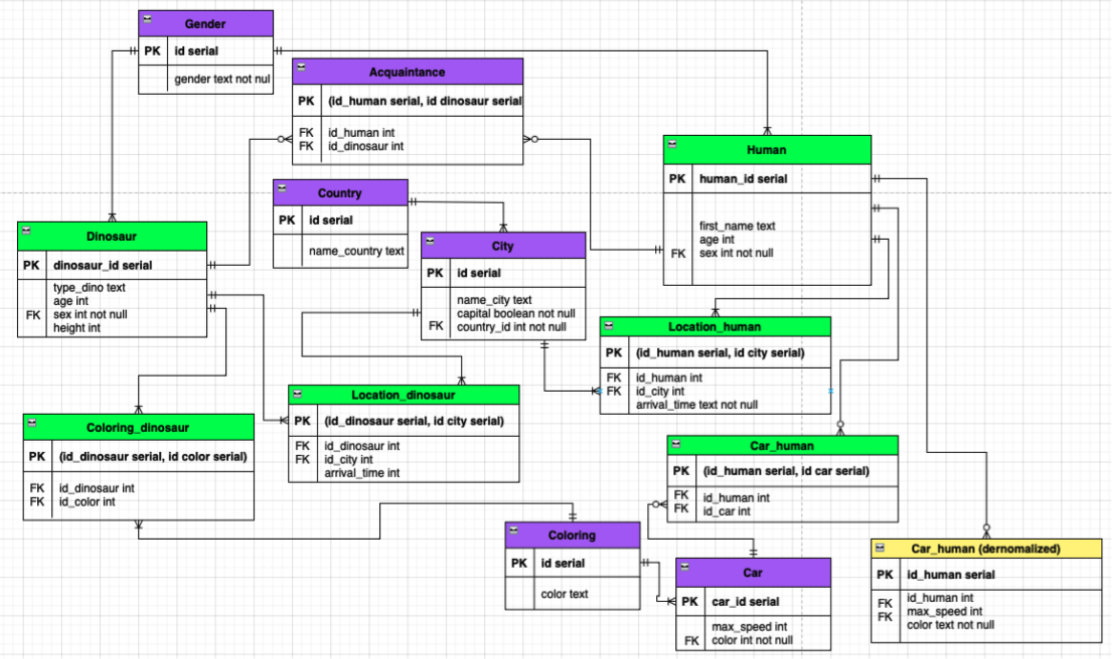
\includegraphics[width=.9\textwidth]{123}